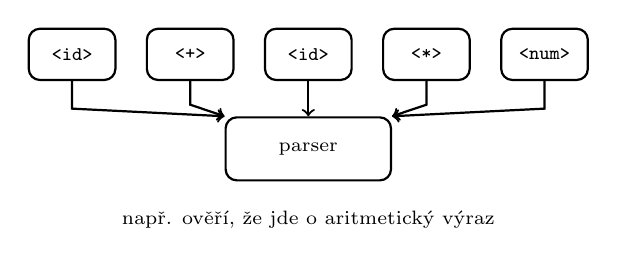
\begin{tikzpicture}[
    tok/.style={
        draw,
        rounded corners,
        thick,
        align=center,
        minimum width=1.1cm,
        minimum height=0.65cm,
        font=\scriptsize
    },
    box/.style={
        draw,
        rounded corners,
        thick,
        align=center,
        minimum width=2.1cm,
        minimum height=0.8cm,
        font=\scriptsize
    },
    arrow/.style={->, thick}
]
    \node<2->[tok] (t1) at (0,0) {\texttt{<id>}};
    \node<2->[tok] (t2) at (1.5,0) {\texttt{<+>}};
    \node<2->[tok] (t3) at (3.0,0) {\texttt{<id>}};
    \node<2->[tok] (t4) at (4.5,0) {\texttt{<*>}};
    \node<2->[tok] (t5) at (6.0,0) {\texttt{<num>}};

    \node<3->[box] (parser) at (3.0,-1.2) {parser};

    \draw<3->[arrow] (t1.south) -- ++(0,-0.35) -- (parser.north west);
    \draw<3->[arrow] (t2.south) -- ++(0,-0.30) -- (parser.north west);
    \draw<3->[arrow] (t3.south) -- (parser.north);
    \draw<3->[arrow] (t4.south) -- ++(0,-0.30) -- (parser.north east);
    \draw<3->[arrow] (t5.south) -- ++(0,-0.35) -- (parser.north east);

    \node<4->[font=\scriptsize, align=center] at (3.0,-2.1)
        {např. ověří, že jde o aritmetický výraz};
\end{tikzpicture}
